\subsection{Searches for other rare and exotic decays}\label{Exotics}
High precision pion decay experiments can access rare and exotic decays, as  demonstrated by
previous experiments (see Fig~\ref{fig:decays}) like PIENU. Extensions of the Standard Model postulate the
existence of additional (sterile) neutrinos \cite{nuMSM}\cite{BrymanShrock}. These additional states can potentially explain
the small mass of the Standard Model neutrinos and contribute to the solution of outstanding puzzles like
the nature of dark matter  and early cosmological processes like small scale structure formation \cite{bertoni}.  
Massive neutrino states $\nu_H$ can be sought in the two-body pion decays
$\pi^+\rightarrow e^+\nu_H$ \cite{Aguilar-Arevalo1} and $\pi^+\rightarrow \mu^+\nu_H$ \cite{Aguilar-Arevalo2}. Exploiting
large datasets of pion decays and the resulting decay muons,  exotic two-body muon decays like $\mu^+\rightarrow e^+X$ can
be sought \cite{Aguilar-Arevalo6}, where X is a massive neutral boson (e.g. an axion or a Majoron).
Similarly, exotic particles have been searched for in three body decays like $\pi^+\rightarrow l^+ \nu X$ ($l=e^+,\mu^+$) \cite{Aguilar-Arevalo8}.
The PIENU experiment also obtained upper limits for the rare decays $\pi^+\rightarrow e^+\nu_e\nu\bar{\nu}$ and
$\pi^+\rightarrow \mu^+\nu_{\mu}\nu\bar{\nu}$ at the $10^6-10^7$ level \cite{Aguilar-Arevalo7}.\\
An experiment with two orders of magnitude more statistics has the potential to improve the existing limits by at least an order of magnitude.
Since the searches are based on a fit to the energy spectra of the visible final state particles, an improved experiment
can bring significant additional advantages in lowering the limits and in reducing the systematic errors. For example, 
the $\pi^+\rightarrow e^+\nu$ low energy tail represents a relevant background for the
$\pi\rightarrow e^+\nu_H$, $\pi^+\rightarrow e^+\nu X$, and $\pi^+\rightarrow e^+\nu_e\nu\bar{\nu}$ searches: 
more precise knowledge of the tail and its further reduction will significantly improve the upper limits beyond the statistics.
The search for rare and exotic decays involving  muons, like $\pi^+\rightarrow \mu^+\nu_H$, $\pi^+\rightarrow \mu^+\nu X$, and $\pi^+\rightarrow \mu^+\nu_{\mu}\nu\bar{\nu}$ will
benefit from an improved stopping target and faster electronics, which will allow better separation of  muons from pions and thus further improve the sensitivity.
Taking into account all the characteristics of an improved pion decay experiment, improvements by more than an order of magnitude can be expected.
\begin{figure}
    \centering
    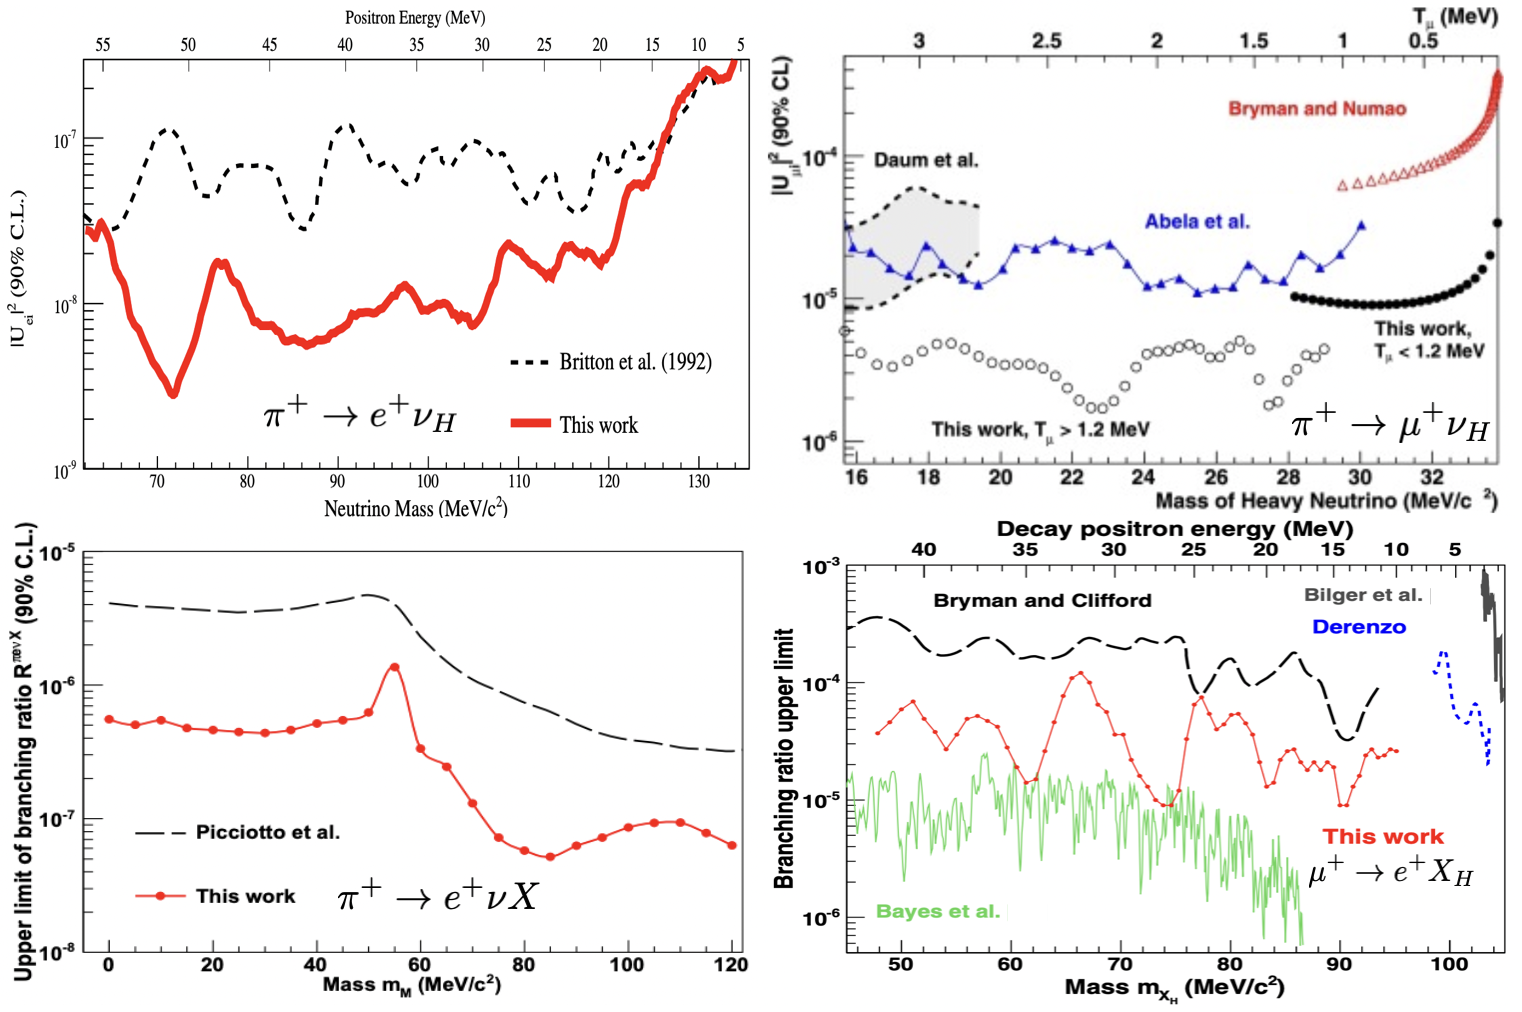
\includegraphics[width=0.6\textwidth]{sections/figures/RareResults.png}
    \caption{Exotic decay searches from the PIENU experiment. The 
    results are indicated with "This work" and show order of magnitude improvements in sensitivity over
    previous experiments.}
    \label{fig:decays}
\end{figure}
